\documentclass[12pt, a4paper, oneside]{article}
\usepackage[utf8]{inputenc}
\usepackage[english, russian]{babel}
\usepackage[T1, T2A]{fontenc}
\usepackage{titlesec}
\usepackage{hyperref}
\usepackage{tikz}
\usepackage[left=4cm,right=2cm,top=4cm,bottom=4cm,bindingoffset=0cm]{geometry}
\usepackage{indentfirst}
\usepackage{graphicx}
\graphicspath{ {./images/} }
\tolerance=10000 % разреженность строки
\hypersetup{
    colorlinks=true,
    linkcolor=black,
    urlcolor=blue,
    citecolor=blue,
}

\title{Thesis}
\author{Evgenia Abdullaeva}
\date{May 2021}

\begin{document}
\begin{titlepage}
    \begin{center}
        Филиал Московского Государственного Университета\\
        имени М.В. Ломоносова в городе Ташкенте\\
        \vspace{0.5cm}
        Факультет прикладной математики и информатики\\
        Кафедра прикладной математики и информатики\\
        \vfill
        Абдуллаева Евгения Гасановна\\
        \vfill
        \textbf{ВЫПУСКНАЯ КВАЛИФИКАЦИОННАЯ РАБОТА\\
        на тему: <<Разработка модулей оповещения и статистики для системы дистанционного обучения>>}\\
        \vspace{0.5cm}
        по направлению 01.03.02 <<Прикладная математика и информатика>>
    \end{center}
    \vfill
    \begin{flushleft}
        Выпускная квалификационная работа рассмотрена и рекомендована к защите\\
        \vspace{0.5cm}
        Руководитель Филиала МГУ имени М.В. Ломоносова в г. Ташкенте\\
        к.ф.-м.н., доцент Строгалов Александр Сергеевич\\
        \vspace{0.5cm}
        Научный руководитель\\
        к.ф.-м.н., в.н.с. Алисейчик Павел Александрович
    \end{flushleft}
    \vfill
    \begin{flushright}
        <<$\rule{1cm}{0.15mm}$>> $\rule{3cm}{0.15mm}$ 2021 г.
    \end{flushright}
    \vfill
    \begin{center}
        Ташкент 2021 г.
    \end{center}
\end{titlepage}

\begin{abstract}
В настоящей работе приведены результаты, достигнутые в процессе расширения функциональности системы дистанционного обучения <<МГУ Контест>>: разработке модуля оповещения пользователей и модуля статистики, а также усовершенствовании раздела помощи пользователям.

В модуле оповещения реализованы возможность подписки пользователя на определенные сущности, оповещение пользователей о событиях на сайте, интерфейс настройки оповещений; переработано отображение списка оповещений. В модуле статистики усовершенствована страница профиля студента, добавлено отображение сведений об активности и успеваемости отдельного студента, а также рейтинг студентов; в список курсов внедрено отображение сведений о сложности курсов. Реализована основная страница раздела помощи пользователям.
\end{abstract}
\selectlanguage{english}
\begin{abstract}
This paper presents the results achieved in the process of expanding the functionality of the “MSU Contest” distance learning system: developing a user notification module and a statistics module, as well as improving the user help section.

The notification module implements the ability to subscribe a user to certain entities, notify users about events on the site, an interface for configuring notifications; redesigned display of the list of notifications. In the statistics module, the student profile page has been improved, the display of information about the activity and progress of an individual student, as well as the rating of students has been added; the display of information about the complexity of courses has been implemented in the list of courses. The main page of the user help section has been implemented.
\end{abstract}
\selectlanguage{russian}
\setcounter{page}{2}
\newpage

\tableofcontents
\newpage

\section{Введение}
\paragraph{} % Постановка проблемы, цель работы
\paragraph{} % Актуальность
\newpage

\section{Общая структура и организация работы}
Данная работа содержит две основные части, описанные в главах 3 и 4. В главе 3 представлено описание работы, проделанной над модулем оповещений, в главе 4 – описание работы над модулем статистики системы дистанционного обучения <<МГУ Контест>>. Система реализована с использованием фреймворка для веб-приложений Django \cite{django}, написанного на языке программирования Python \cite{python}, в связи с этим расширение функциональности системы также производится с использованием указанных технологий.

В модуле статистики для реализации графического отображения собранных сведений используется инструмент Chart.js \cite{chartjs}.
\newpage

\section{Модуль оповещения}
\subsection{Подписка на оповещения}
Персонализация оповещений о событиях на сайте требует реализации механизма подписки пользователей на определенные сущности, о состоянии которых пользователь желает получать оповещения. Поэтому для предоставления преподавателям возможности получать оповещения о новых комментариях и посылках лишь к определенным курсам и разделам была реализована подписка пользователя на курсы и разделы.

На детальной странице каждого курса реализован интерфейс, доступный преподавателям, предоставляющий возможность подписаться на данный курс или отписаться от курса, а также подписаться на данный курс и все его разделы или отписаться от них. На детальной странице каждого раздела реализован интерфейс, доступный преподавателям, позволяющий подписаться на данный раздел или отписаться от него.

Все пользователи имеют возможность подписаться на оповещения об объявлениях и о расписании. Такую возможность предоставляет интерфейс настройки оповещений, реализация которого описана ниже.
\subsection{Оповещения о событиях на сайте}
Для пользователей сайта реализована возможность получать оповещения о следующих событиях:
\begin{itemize}
    \item [-] о добавлении комментария к курсу, разделу, задаче или посылке – оповещения получают преподаватели, подписанные на курс или раздел, к которым написан данный комментарий, если же комментарий написан к задаче или посылке к задаче, то оповещения получают преподаватели, подписанные на раздел, включающий данную задачу;
    \item [-] о новой посылке к задаче – оповещения получают преподаватели, подписанные на раздел, включающий задачу, к которой отправлена посылка;
    \item [-] о публикации объявления – оповещения получают все пользователи, находящиеся в группе, которой адресовано объявление, и подписанные на оповещения об объявлениях;
    \item [-] о добавлении расписания – оповещения получают все пользователи, подписанные на оповещения о расписании;
    \item [-] о создании вопроса – оповещение получает преподаватель, которому адресован вопрос, при переадресации вопроса или при появлении ответа на вопрос, оповещение об этом получает пользователь, задавший данный вопрос;
    \item [-] о сообщении об ошибке – оповещения получают администраторы сайта, при изменении статуса сообщения оповещение получает пользователь, отправивший сообщение об ошибке.
\end{itemize}
% \subsection{Динамическая отметка комментариев как прочтенных}
\subsection{Список оповещений}
\subsubsection{Бесконечная прокрутка списка оповещений}
Для списка оповещений пользователя реализован механизм динамического раскрытия списка при прокручивании. При переходе на страницу списка оповещений отображаются лишь последние 30 полученных пользователем оповещений, при прокручивании страницы к концу отображаемого списка подгружаются следующие 30 более давних оповещений.
\subsubsection{Динамическая отметка оповещений как прочтенных}
В списке оповещений еще не прочтенные пользователем оповещения помечаются специальным цветом. При их просмотре в списке, то есть при нахождении таких оповещений в области видимости пользователя, они динамически помечаются как прочтенные, а также динамически обновляется значение счетчика непрочтенных оповещений. При просмотре объектов непрочтенных оповещений, например, комментария или объявления, о добавлении которых были получены данные оповещения, данные оповещения также помечаются как прочтенные.
\subsection{Интерфейс настройки оповещений}
\subsubsection{Выбор типов получаемых оповещений}
\begin{center}
    
\includegraphics[scale=0.4]{activity-settings}
\end{center}

Пользователям предоставляется возможность выбора типов получаемых оповещений. Для этого реализован интерфейс настройки оповещений, где пользователь может отметить некоторые из следующих пунктов:
\begin{itemize}
    \item [-] объявления – доступен всем пользователям;
    \item [-] расписание – доступен всем пользователям;
    \item [-] комментарии – доступен преподавателям;
    \item [-] посылки – доступен преподавателям.
\end{itemize}

При подписке на оповещения о комментариях или посылках при отсутствии у пользователя подписок на курсы или разделы, пользователь подписывается на все курсы и разделы. При отписке от оповещений о комментариях и посылках пользователь, соответственно, отписывается от всех курсов и разделов.
\subsubsection{Список подписок на курсы и разделы}
\begin{center}
    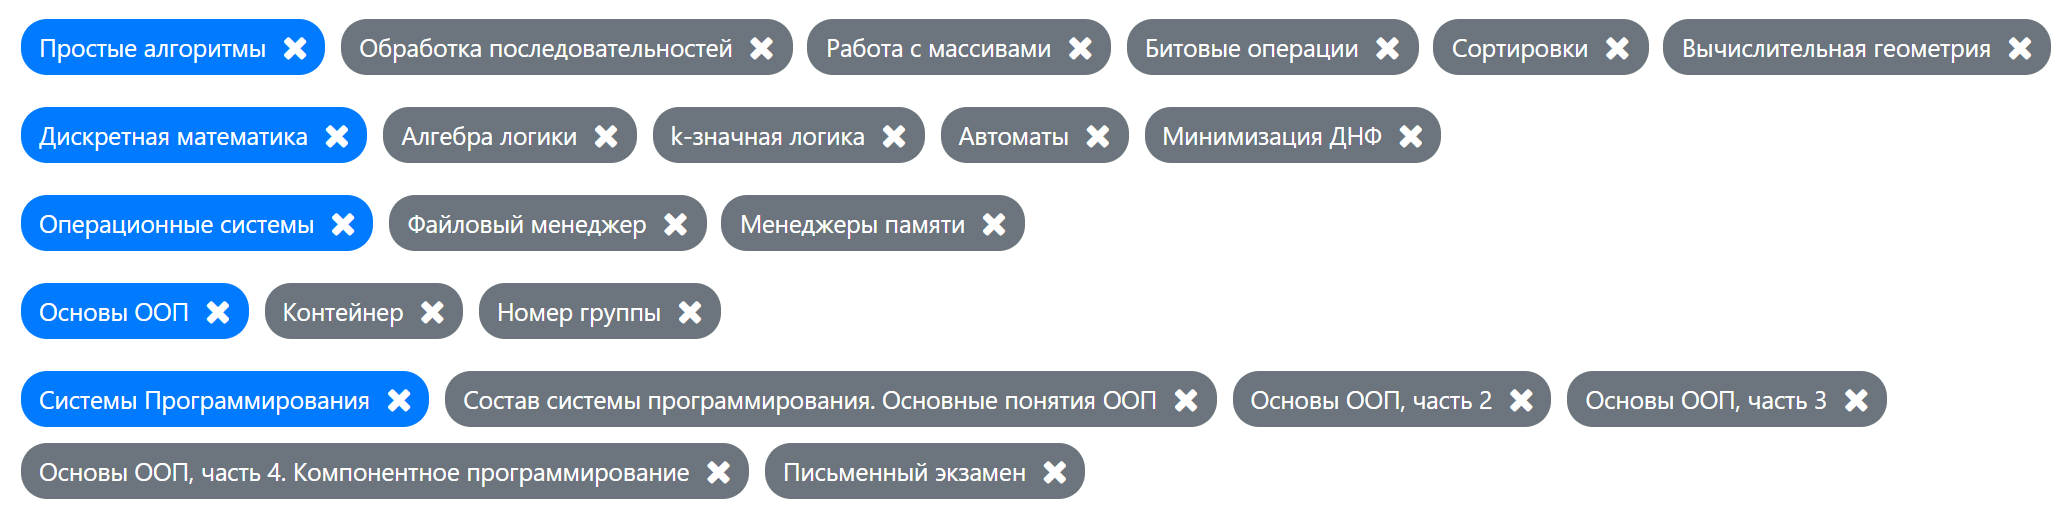
\includegraphics[scale=0.25]{courses-contests-subscriptions}
\end{center}

Интерфейс настройки оповещений включает также интерактивный список курсов и разделов, на которые подписан пользователь. Данный раздел интерфейса настройки оповещений реализован так, что по нажатию на элемент списка (курс или раздел) пользователь имеет возможность отписаться от выбранного курса или раздела. Список доступен преподавателям.
\newpage

\section{Модуль статистики}
\subsection{Профиль студента}
\subsubsection{Персонализированные изображения профиля}
С целью усовершенствования отображения профиля пользователя реализована генерация персонализированных изображений профиля с инициалами имени и фамилии пользователя. Полученные изображения также отображаются в списке комментариев перед именем пользователя.
\subsubsection{Сведения об активности}
\begin{center}
    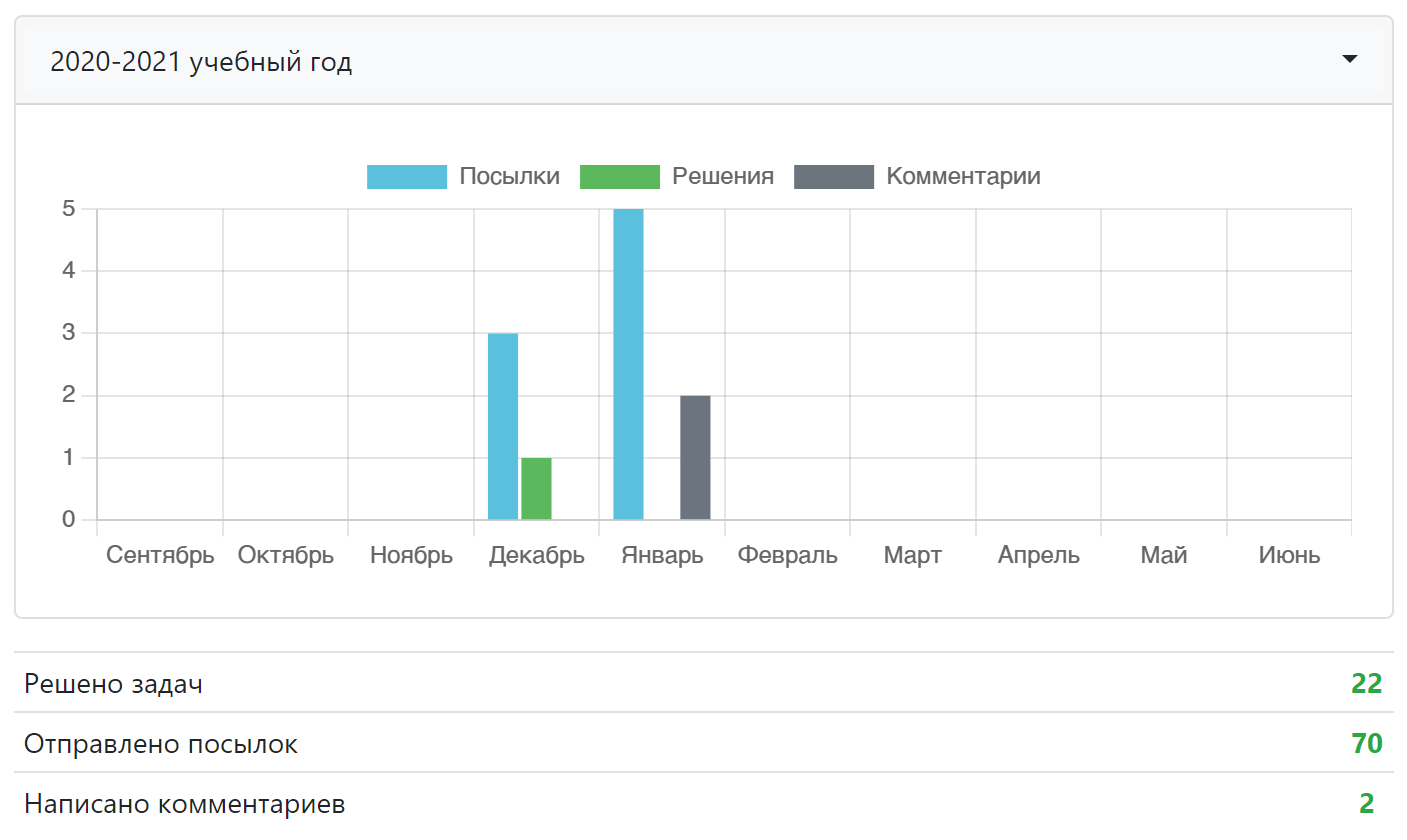
\includegraphics[scale=0.25]{account-activity}
\end{center}

Реализовано отображение сведений об активности студента в виде столбчатой диаграммы, где по месяцам указаны количество посылок, сделанных студентом, количество решенных задач и количество комментариев. Имеется возможность выбрать для просмотра определенный учебный год или все время.

Также в сведениях об активности студента отображается общее количество решенных задач, посылок и комментариев студента.
\subsubsection{Результаты курсов}
Реализовано отображение результатов курсов, пройденных студентом, в профиле студента. Для каждого курса отображается уровень, ссылка на страницу с детальными результатами курса и оценка по данному курсу.

На странице с детальными результатами курса отображаются количества посылок к каждой из задач курса, оценки за каждую задачу курса, а также результаты решений задач, не входящих в обязательное задание студента по данному курсу, а решенных студентом дополнительно. Также здесь отображается в процентах в виде шкалы прогресса точность студента по данному курсу, подробности расчета которой описаны ниже.
\subsubsection{Подсчет общей успеваемости и точности студента}
Подсчет общей успеваемости студентов реализован на основании оценок студентов по пройденным курсам. Общая успеваемость отображается в процентах в виде шкалы прогресса в профиле студента.

Подсчет точности студента реализован на основании количества посылок к задаче до первой успешной, то есть до посылки, считающейся решением задачи. Пронумеруем все решенные студентом задачи от 1 до $n$, где $n$ – общее количество решенных студентом задач. Тогда для каждой решенной студентом задачи с номером $i$ точность $A_i$ рассчитывается следующим образом: 
$$A_i=\frac{100\%}{\lceil \frac{C_i}{L_i}\rceil},$$
где $C_i$ – количество посылок к данной задаче до успешной, $L_i$ – разрешенное количество посылок к данной задаче. Точность $A$ студента является средней точностью этого студента по каждой из решенных задач, то есть
$$A=\frac{1}{n}\sum_{i=1}^{n}A_i.$$

Точность студента по отдельному курсу рассчитывается аналогично на основании количества посылок до первой успешной к каждой из задач данного курса.

Точность профиле студента отображается в процентах в виде шкалы прогресса.
\subsection{Рейтинг студентов}
На основании общей успеваемости студентов реализовано отображение рейтинга студентов указанного уровня, всех студентов, выпускников и отчисленных студентов. На основании успеваемости студентов по отдельным курсам реализовано отображение рейтинга студентов указанного уровня, всех студентов, выпускников и отчисленных студентов по данным курсам.

Отображение рейтинга студентов по общей успеваемости доступно всем преподавателям, по успеваемости по отдельным курсам – доступно преподавателям, ведущим соответствующие курсы.
\subsection{Сведения о сложности курсов}
\begin{center}
    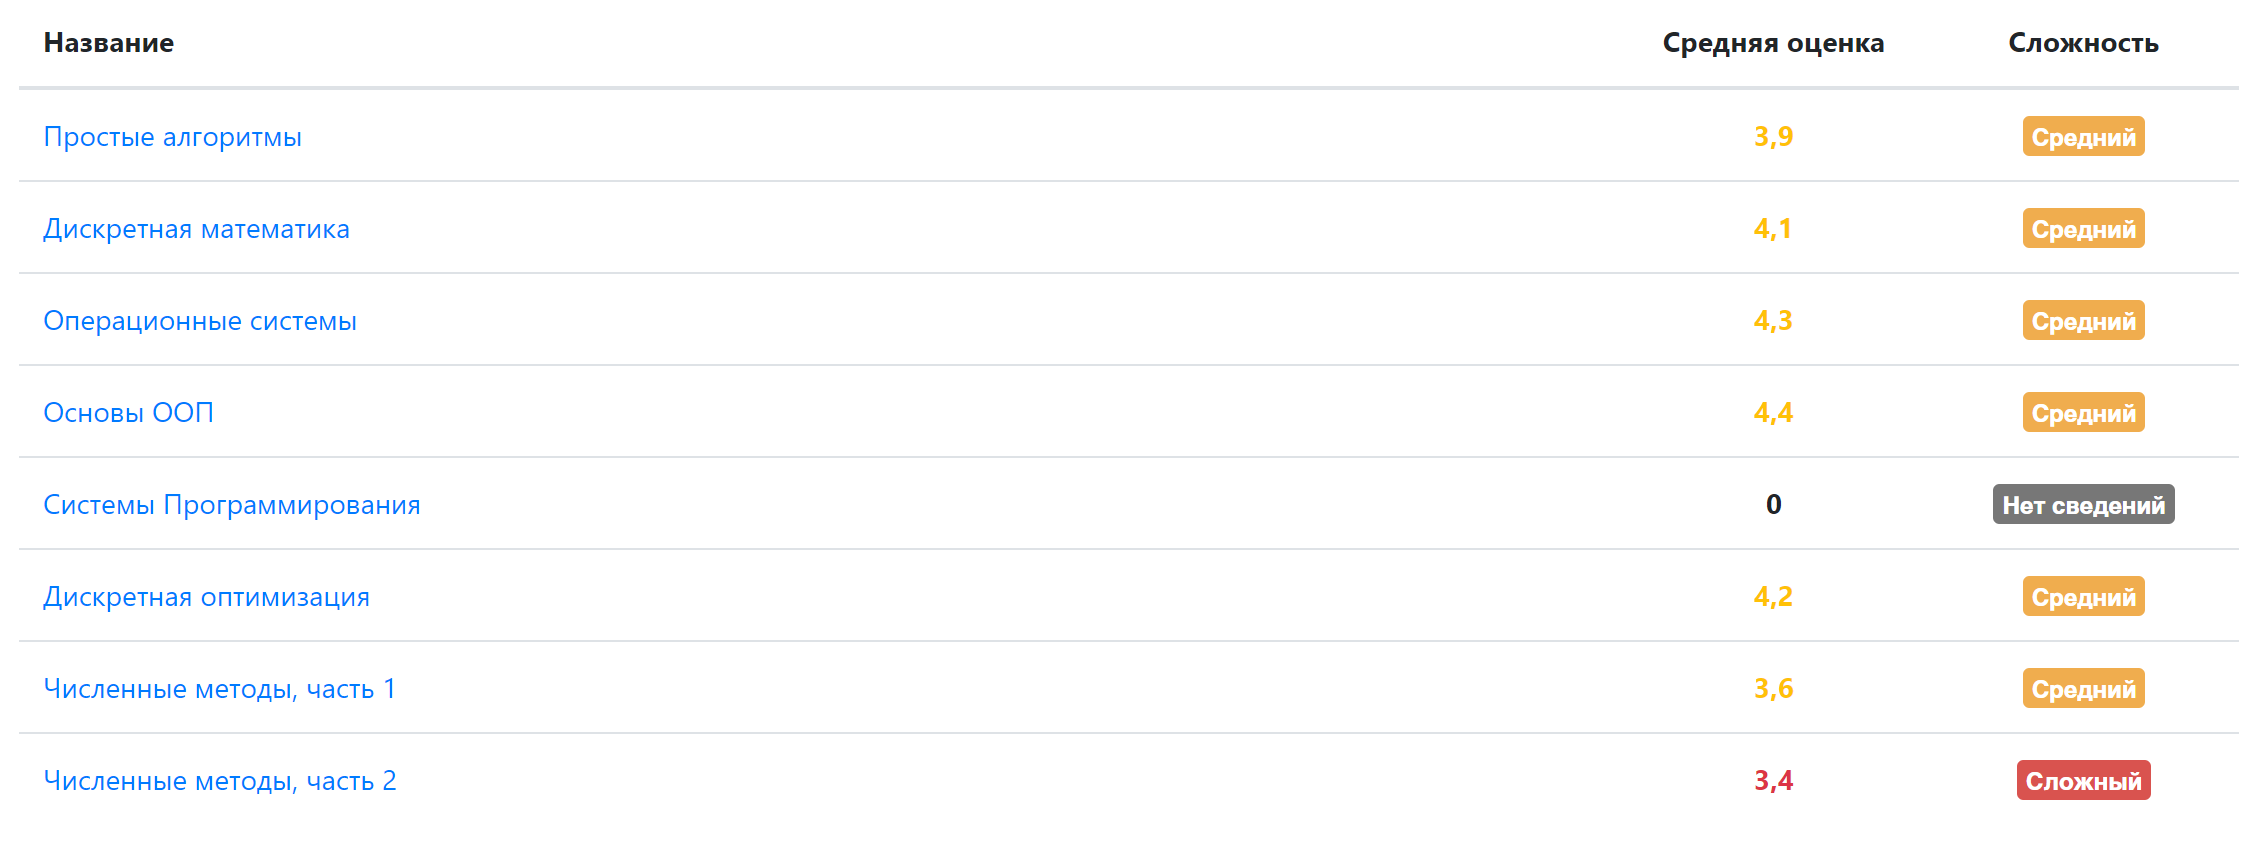
\includegraphics[scale=0.25]{course-difficulty}
\end{center}

Для преподавателей в списке курсов, которые преподаватели ведут, реализовано отображение сведений о сложности данных курсов. Сложность курса определяется на основании средней оценки студентов, завершивших данный курс. В случае, если средняя оценка студентов по пятибалльной шкале составляет не менее 4.5 баллов, курс считается легким; иначе, в случае средней оценки студентов не менее 3.5 баллов, курс считается средним по сложности; иначе, в случае средней оценки студентов не менее 2-х баллов, курс считается сложным. Также в списке курсов отображается и средняя оценка студентов по каждому курсу.
\newpage

\section{Раздел помощи}
\begin{center}
    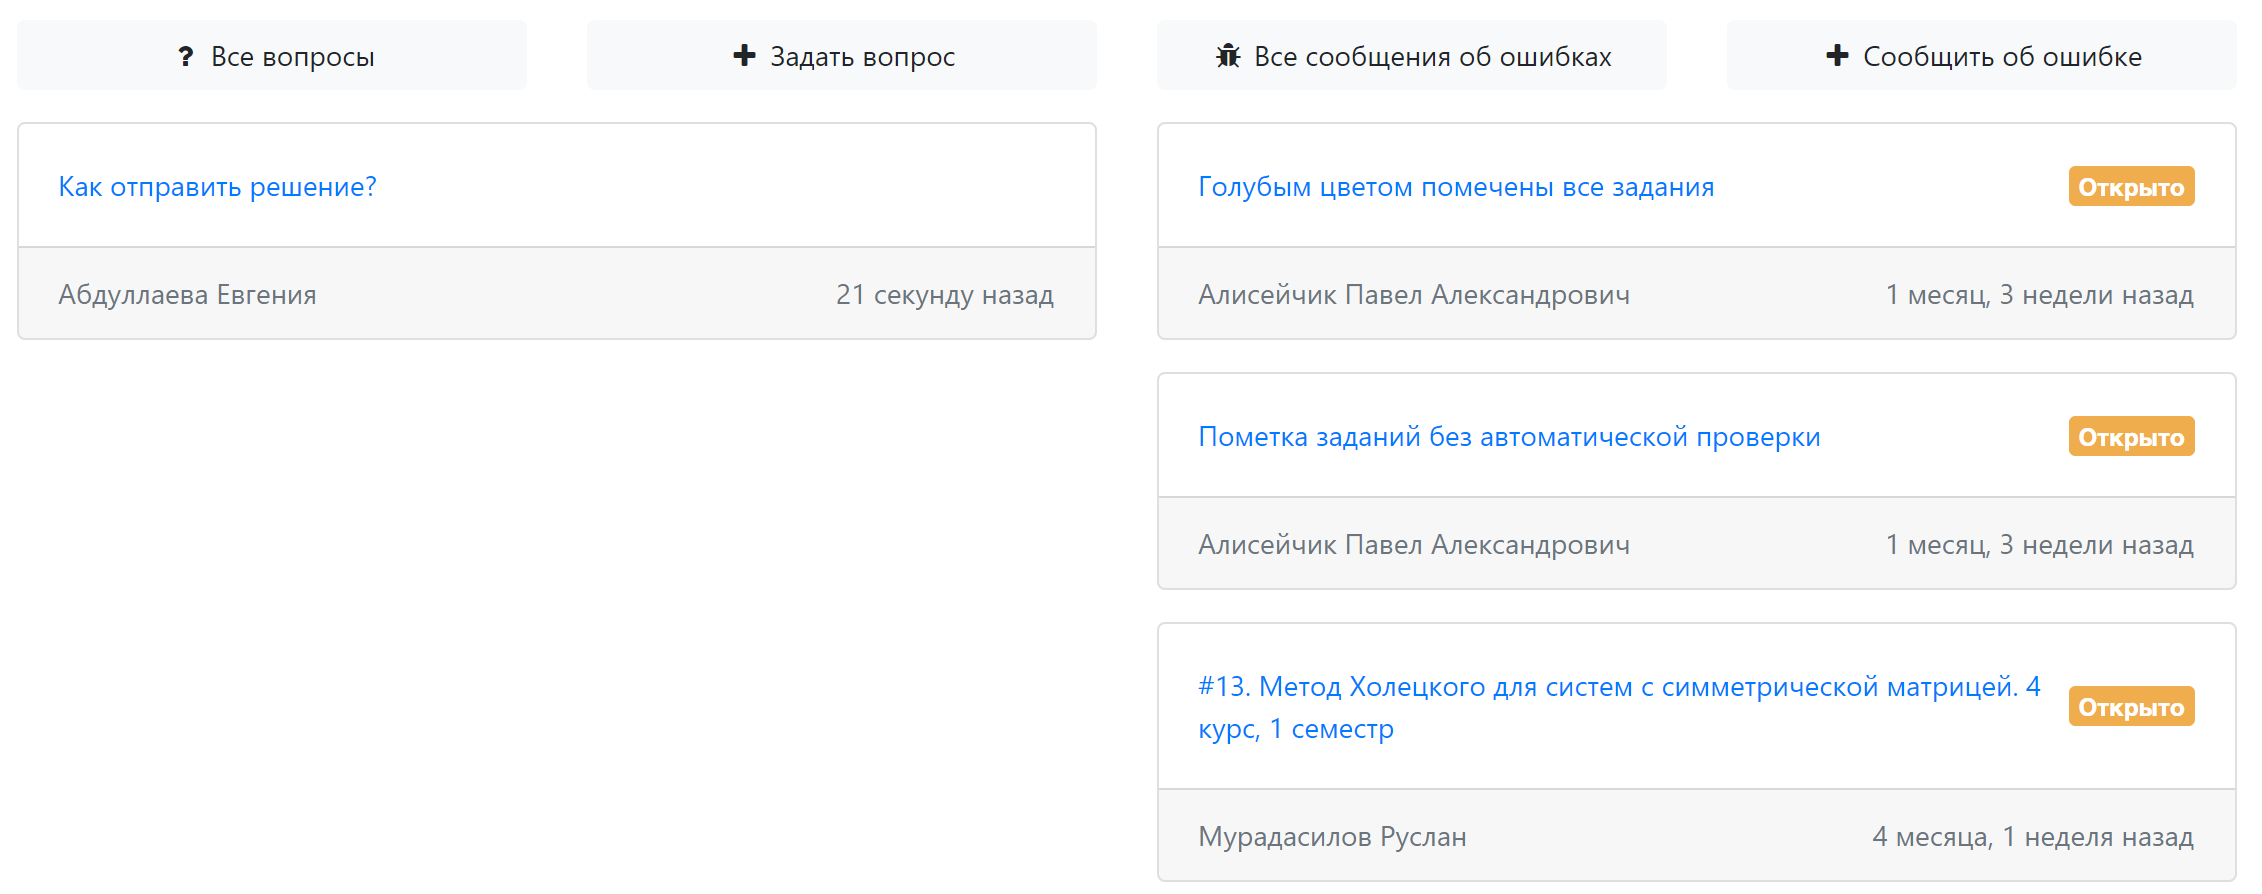
\includegraphics[scale=0.25]{support}
\end{center}

В разделе помощи модели вопроса добавлено необязательное поле адресата для предоставления пользователям возможности задать вопрос конкретному преподавателю, соответственно переработана форма создания вопроса.

Реализована основная страница раздела помощи пользователям. На рассматриваемой странице для студента в виде карточек отображается список из пяти наиболее новых опубликованных или заданных данным студентом вопросов и список сообщений об ошибках со статусом <<открыто>>, отправленных данным студентом; также на этой странице присутствуют ссылки в виде кнопок, позволяющие задать вопрос, отправить сообщение об ошибке, перейти к списку всех опубликованных или заданных этим студентом вопросов или списку всех отправленных студентом сообщений об ошибках. Для преподавателя и администратора на странице в виде карточек отображается список вопросов, у которых пока отсутствует ответ и список сообщений об ошибках со статусом <<открыто>>; также на этой странице присутствуют ссылки в виде кнопок, позволяющие задать вопрос, отправить сообщение об ошибке, перейти к списку всех вопросов или списку всех сообщений об ошибках.
\newpage

\section{Заключение}
В рамках настоящей работы был реализован модуль оповещения пользователей и модуль статистики для системы дистанционного обучения <<МГУ Контест>>, а также усовершенствован раздел помощи пользователям системы. Таким образом была расширена функциональность системы дистанционного обучения <<МГУ Контест>>.
\newpage

\section{Приложения}
\subsection{Модель подписки}
\begin{verbatim}
class SubscriptionManager(models.Manager):
    def make_subscription(self, user, object, cascade=False):
        Course = apps.get_model('contests', 'Course')
        Contest = apps.get_model('contests', 'Contest')
        Submission = apps.get_model('contests', 'Submission')
        Subscription(object=object, user=user).save()
        if isinstance(object, Course) and cascade:
            subscribed_contest_ids = \
                Subscription.objects.for_user_model(user, Contest) \
                    .values_list('object_id', flat=True)
            new_contest_ids = \
                Contest.objects.filter(course=object) \
                    .exclude(id__in=subscribed_contest_ids) \
                        .values_list('id', flat=True)
            contest_subscriptions = (Subscription(
                    object_type=ContentType.objects.get_for_model(Contest), 
                    object_id=contest_id, user=user
                ) for contest_id in new_contest_ids)
            Subscription.objects.bulk_create(contest_subscriptions)
        if isinstance(object, (Course, Contest)):
            if not Subscription.objects. \
                for_user_models(user, Comment, Submission).exists():
                Subscription(object_type=ContentType.objects. \
                    get_for_model(model=Comment), user=user).save()
                Subscription(object_type=ContentType.objects. \
                    get_for_model(model=Submission), user=user).save()
    
    def delete_subscription(self, user, object, cascade=False):
        Course = apps.get_model('contests', 'Course')
        Contest = apps.get_model('contests', 'Contest')
        Submission = apps.get_model('contests', 'Submission')
        Subscription.objects.for_user_object(user, object).delete()
        if isinstance(object, Course) and cascade:
            course_contest_ids = \
                Contest.objects.filter(course=object) \
                    .values_list('id', flat=True)
            Subscription.objects.for_user_model(user, Contest) \
                .filter(object_id__in=course_contest_ids).delete()
        if not Subscription.objects \
            .for_user_models(user, Course, Contest).exists():
            Subscription.objects \
                .for_user_models(user, Comment, Submission).delete()

class SubscriptionQuerySet(models.QuerySet):
    def for_user_model(self, user, model):
        return self.filter(user=user, 
            object_type=ContentType.objects.get_for_model(model))

    def for_user_models(self, user, *models):
        return self.filter(user=user, 
            object_type__in=ContentType.objects \
                .get_for_models(*models).values())
    
    def for_user_object(self, user, object):
        return self.filter(user=user, 
            object_type=ContentType.objects \
                .get_for_model(object._meta.model),
            object_id=object.id)

class Subscription(models.Model):
    object_type = models.ForeignKey(ContentType, on_delete=models.CASCADE)
    object_id = models.PositiveIntegerField(null=True, blank=True)
    object = GenericForeignKey(ct_field='object_type')
    user = models.ForeignKey(User, on_delete=models.CASCADE)
    objects = SubscriptionManager.from_queryset(SubscriptionQuerySet)()

    class Meta:
        verbose_name = "Подписка"
        verbose_name_plural = "Подписки"
        unique_together = ('user', 'object_type', 'object_id')

    def validate_unique(self, exclude=None):
        if Subscription.objects.exclude(id=self.id).filter(
            user=self.user, 
            object_type=self.object_type, 
            object_id__isnull=True).exists():
            raise ValidationError("Подписка с такими значениями полей \
                User, Object type и Object id уже существует.")
        super().validate_unique(exclude)

    def __str__(self):
        return '%s, %s%s' % (self.user.account.get_full_name(), 
            self.object_type.model,
            ': ' + self.object.title if self.object_id is not None else '')
\end{verbatim}
\newpage

\section{Список использованных источников и литературы}
\begingroup
\renewcommand{\section}[2]{}
\begin{thebibliography}{20}
    \bibitem{msu-article-1}
    Моделирование процесса обучения / В. Б. Кудрявцев, П. А. Алисейчик, К. Вашик, Ж. Кнап, А. С. Строгалов, С. Г. Шеховцов // Интеллектуальные системы. – 2006, т. 10, вып. 1-4, стр. 189-270.
    \bibitem{msu-article-2}
    О дистанционном образовании – пример реализации и перспективы / П. А. Алисейчик, А. С. Строгалов, Р. А. Бекташев // Интеллектуальные системы. Теория и приложения. – 2016, т. 20, вып. 3, стр. 127-133.
    \bibitem{msu-contest}
    Репозиторий проекта <<МГУ Контест>>\\
    \url{https://github.com/ruslanbektashev/contest}
    \bibitem{django}
    Документация фреймворка Django\\
    \url{https://docs.djangoproject.com/en/3.0}
    \bibitem{python}
    Документация языка Python\\
    \url{https://docs.python.org/3}
    \bibitem{chartjs}
    Документация инструмента Chart.js\\
    \url{https://www.chartjs.org/docs/latest/}
\end{thebibliography}
\endgroup

\end{document}
